\documentclass[11pt]{article}
\usepackage{amsmath}
\usepackage{amssymb}
\usepackage{graphicx}
\usepackage{tabularx}
\usepackage{fancyhdr}
\usepackage{lastpage}

% Page layout
\usepackage[top=1in, bottom=1in, left=1in, right=1in]{geometry}

% Header and footer
\pagestyle{fancy}
\fancyhf{}
\rfoot{Page \thepage}
\renewcommand{\headrulewidth}{0pt}

% Modified Question command with left-aligned number
\newcommand{\questiona}[2]{
    \noindent\textbf{Q#2.} #1 \hfill \textbf{[1 Mark]}
}

\newcommand{\questionb}[2]{
    \noindent\textbf{Q#2.} #1 \hfill \textbf{[2 Marks]}
}

\begin{document}

% Title section with horizontal line
\begin{center}
    \Large\textbf{GATE 2017 - Biotechnology (BT)} \\
    \large\textbf{General Aptitude and Technical Questions} \\
    \rule{\textwidth}{0.5pt} % Horizontal line below heading
\end{center}

\vspace{0.5cm}

% General Aptitude Section
\section*{General Aptitude}

\questiona{She has a sharp tongue and it can occasionally turn \_\_\_\_\_.}{1}
\begin{enumerate}
    \item[(A)] hurtful
    \item[(B)] left  
    \item[(C)] methodical
    \item[(D)] vital
\end{enumerate}

\vspace{0.5cm}

\questiona{I \_\_\_\_\_ made arrangements had I \_\_\_\_\_ informed earlier.}{2}
\begin{enumerate}
    \item[(A)] could have, been
    \item[(B)] would have, being  
    \item[(C)] had, have
    \item[(D)] had been, been
\end{enumerate}

\vspace{0.5cm}

\questiona{In the summer, water consumption is known to decrease overall by 25\%. A Water Board official states that in the summer household consumption decreases by 20\%, while other consumption increases by 70\%. Which of the following statements is correct?}{3}
\begin{enumerate}
    \item[(A)] The ratio of household to other consumption is 8/17
    \item[(B)] The ratio of household to other consumption is 1/17  
    \item[(C)] The ratio of household to other consumption is 17/8
    \item[(D)] There are errors in the official's statement.
\end{enumerate}

\vspace{0.5cm}

\questiona{40\% of deaths on city roads may be attributed to drunken driving. The number of degrees needed to represent this as a slice of a pie chart is}{4}
\begin{enumerate}
    \item[(A)] 120
    \item[(B)] 144  
    \item[(C)] 160
    \item[(D)] 212
\end{enumerate}

\vspace{0.5cm}

\questiona{Some tables are shelves. Some shelves are chairs. All chairs are benches. Which of the following conclusions can be deduced from the preceding sentences?
\begin{enumerate}
    \item[i.] At least one bench is a table
    \item[ii.] At least one shelf is a bench
    \item[iii.] At least one chair is a table
    \item[iv.] All benches are chairs
\end{enumerate}}{5}
\begin{enumerate}
    \item[(A)] Only i
    \item[(B)] Only ii  
    \item[(C)] Only ii and iii
    \item[(D)] Only iv
\end{enumerate}

\hspace{0.5cm}

\questionb{"If you are looking for a history of India, or for an account of the rise and fall of the British Raj, or for the reason of the cleaving of the subcontinent into two mutually antagonistic parts and the effects this mutilation will have in the respective sections, and ultimately on Asia, you will not find it in these pages; for though I have spent a lifetime in the country, I lived too near the seat of events, and was too intimately associated with the actors, to get the perspective needed for the impartial recording of these matters".

Here, the word 'antagonistic' is closest in meaning to}{6}
\begin{enumerate}
    \item[(A)] impartial
    \item[(B)] argumentative  
    \item[(C)] separated
    \item[(D)] hostile
\end{enumerate}

\vspace{0.5cm}

\questionb{S, T, U, V, W, X, Y, and Z are seated around a circular table. T's neighbours are Y and V. Z is seated third to the left of T and second to the right of S. U's neighbours are S and Y; and T and W are not seated opposite each other. Who is third to the left of V?}{7}
\begin{enumerate}
    \item[(A)] X
    \item[(B)] W  
    \item[(C)] U
    \item[(D)] T
\end{enumerate}

\vspace{0.5cm}

\questionb{Trucks (10 m long) and cars (5 m long) go on a single lane bridge. There must be a gap of at least 20 m after each truck and a gap of at least 15 m after each car. Trucks and cars travel at a speed of 36 km/h. If cars and trucks go alternately, what is the maximum number of vehicles that can use the bridge in one hour?}{8}
\begin{enumerate}
    \item[(A)] 1440
    \item[(B)] 1200  
    \item[(C)] 720
    \item[(D)] 600
\end{enumerate}

\vspace{0.5cm}

\questionb{There are 3 Indians and 3 Chinese in a group of 6 people. How many subgroups of this group can we choose so that every subgroup has at least one Indian?}{9}
\begin{enumerate}
    \item[(A)] 56
    \item[(B)] 52  
    \item[(C)] 48
    \item[(D)] 44
\end{enumerate}

\vspace{0.5cm}

\questionb{A contour line joins locations having the same height above the mean sea level. The following is a contour plot of a geographical region. Contour lines are shown at 25 m intervals in this plot.

\begin{center}
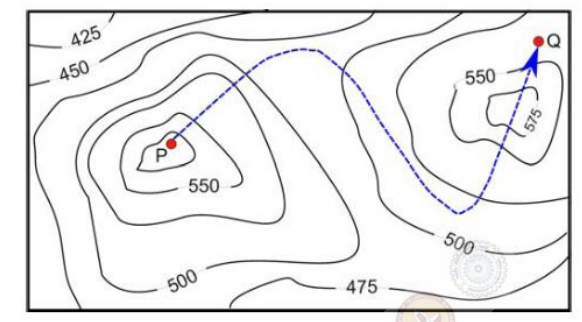
\includegraphics[width=0.5\textwidth]{figures/10.png}
\end{center}

The path from P to Q is best described by}{10}
\begin{enumerate}
    \item[(A)] Up-Down-Up-Down
    \item[(B)] Down-Up-Down-Up  
    \item[(C)] Down-Up-Down
    \item[(D)] Up-Down-Up
\end{enumerate}

\vspace{1 cm}

\section*{Technical Section}

\questiona{An enzyme catalyzes a reaction by}{1}
\begin{enumerate}
    \item[(A)] decreasing the energy of the substrate.
    \item[(B)] decreasing the activation energy of the reaction.  
    \item[(C)] decreasing product stability.
    \item[(D)] increasing the activation barrier of the reaction.
\end{enumerate}

\vspace{0.5cm}

\questiona{Natural proteins are composed primarily of 20 $\alpha$-amino acids. Which one of the following statements is true for any of these amino acids in a solution of pH 1.5?}{2}
\begin{enumerate}
    \item[(A)] Only the amino group is ionized.
    \item[(B)] Only the carboxylic acid group is ionized.  
    \item[(C)] Both amino and carboxylic acid groups are ionized.
    \item[(D)] Both amino and carboxylic acid groups are neutral.
\end{enumerate}

\vspace{0.5cm}

\questiona{Which one of the following organisms is an indicator of fecal contamination?}{3}
\begin{enumerate}
    \item[(A)] Escherichia coli
    \item[(B)] Streptococcus lactis  
    \item[(C)] Bacillus subtilis
    \item[(D)] Lactobacillus acidophilus
\end{enumerate}

\vspace{0.5cm}

\questiona{The surface area (in m$^2$) of the largest sphere that can fit into a hollow cube with edges of length 1 meter is \_\_\_\_\_.}{4}

\vspace{0.5cm}

\questiona{In a thin layer chromatography experiment using a silica gel plate, a compound showed migration of 12.5 cm and the solvent front showed migration of 18 cm. The $R_f$ value for the compound is \_\_\_\_\_.}{5}

\vspace{0.5cm}

\questiona{$\lim_{x \to 0} \frac{\sin(x)}{x}$}{6}

\vspace{0.5cm}

\questiona{Which one of the following mechanisms is used by human pathogens to evade host immune responses?}{7}
\begin{enumerate}
    \item[(A)] Somatic hypermutation
    \item[(B)] Antibody production  
    \item[(C)] Antigenic variation
    \item[(D)] Complement activation
\end{enumerate}

\vspace{0.5cm}

\questiona{If the nucleotide composition (\%) of a viral genome is $A = 10$, $U = 20$, $C = 40$, and $G = 30$, which one of the following is this genome?}{8}
\begin{enumerate}
    \item[(A)] Double stranded RNA
    \item[(B)] Single stranded RNA  
    \item[(C)] Single stranded DNA
    \item[(D)] Double stranded DNA
\end{enumerate}

\vspace{0.5cm}

\questiona{Which one of the following techniques can be used to determine the structure of a 15 kDa globular protein at atomic resolution?}{9}
\begin{enumerate}
    \item[(A)] Raman spectroscopy
    \item[(B)] IR spectroscopy  
    \item[(C)] UV spectroscopy
    \item[(D)] NMR spectroscopy
\end{enumerate}

\vspace{0.5cm}

\questiona{Assertion [a]: Gram negative bacteria show staining with saffranin. Reason [r]: Gram negative bacteria have an outer membrane with lipopolysaccharides.}{10}
\begin{enumerate}
    \item[(A)] Both [a] and [r] are true and [r] is the correct reason for [a].
    \item[(B)] Both [a] and [r] are true but [r] is not the correct reason for [a].  
    \item[(C)] Both [a] and [r] are false.
    \item[(D)] [a] is true but [r] is false.
\end{enumerate}

\vspace{0.5cm}

\questiona{The plant hormone indole-3-acetic acid is derived from}{11}
\begin{enumerate}
    \item[(A)] histidine
    \item[(B)] tyrosine  
    \item[(C)] tryptophan
    \item[(D)] proline
\end{enumerate}

\vspace{0.5cm}

\questiona{Enzyme-linked immunosorbent assay (ELISA) is used for}{12}
\begin{enumerate}
    \item[(A)] quantifying antibody levels in blood
    \item[(B)] determining the molecular weight of an antigen  
    \item[(C)] purifying proteins from biological fluids
    \item[(D)] determining the molecular weight of an antibody
\end{enumerate}

\vspace{0.5cm}

\questiona{Macrophages eliminate pathogenic bacteria upon activation by}{13}
\begin{enumerate}
    \item[(A)] NK cells
    \item[(B)] basophils  
    \item[(C)] CD4+ T cells
    \item[(D)] plasma cells
\end{enumerate}

\vspace{0.5cm}

\questiona{If a protein contains four cysteine residues, the number of different ways they can simultaneously form two intra-molecular disulphide bonds is \_\_\_\_\_.}{14}

\vspace{0.5cm}

\questiona{Secretory proteins synthesized by ER-associated ribosomes traverse through}{15}
\begin{enumerate}
    \item[(A)] mitochondria
    \item[(B)] peroxisomes  
    \item[(C)] the Golgi apparatus
    \item[(D)] the nucleus
\end{enumerate}

\vspace{0.5cm}

\questiona{For $y = f(x)$, if $\frac{d^2 y}{dx^2} = 0$, $\frac{dy}{dx} = 0$ at $x = 0$, and $y = 1$ at $x = 1$, the value of $y$ at $x = 2$ is \_\_\_\_\_.}{16}

\vspace{0.5cm}

\questiona{During protein synthesis, tRNAs are NOT involved in}{17}
\begin{enumerate}
    \item[(A)] charging
    \item[(B)] initiation  
    \item[(C)] elongation
    \item[(D)] termination
\end{enumerate}

\vspace{0.5cm}

\questiona{In eukaryotes, cytokinesis is inhibited by}{18}
\begin{enumerate}
    \item[(A)] cytochalasin D
    \item[(B)] vinblastine  
    \item[(C)] nocodazole
    \item[(D)] colchicine
\end{enumerate}

\vspace{0.5cm}

\questiona{A proto-oncogene is suspected to have undergone duplication in a certain type of cancer. Of the following techniques, which one would verify the gene duplication?}{19}
\begin{enumerate}
    \item[(A)] Northern blotting
    \item[(B)] Southern blotting  
    \item[(C)] South western blotting
    \item[(D)] Western blotting
\end{enumerate}

\vspace{0.5cm}

\questiona{A polymerase chain reaction (PCR) was set up with the following reagents: DNA template, \textit{Taq} polymerase, buffer, dNTPs, and Mg$^{2+}$. Which one of the following is missing in the reaction mixture?}{20}
\begin{enumerate}
    \item[(A)] Helicase
    \item[(B)] Single-stranded binding proteins  
    \item[(C)] Primers
    \item[(D)] Reverse transcriptase
\end{enumerate}

\vspace{0.5cm}

\questiona{An enzymatic reaction exhibits Michaelis-Menten kinetics. For this reaction, on doubling the concentration of enzyme while maintaining [S] $>>$[$E_0$],}{21}
\begin{enumerate}
    \item[(A)] both Km and Vmax will remain the same.
    \item[(B)] Km will remain the same but Vmax will increase.  
    \item[(C)] Km will increase but Vmax will remain the same.
    \item[(D)] both Km and Vmax will increase.
\end{enumerate}

\vspace{0.5cm}

\questiona{A 5 liter chemostat is fed fresh medium at 0.2 liters/minute having a substrate concentration of 25 grams/liter. At steady state, the outgoing stream has substrate concentration of 2.5 grams/liter. The rate of consumption (grams/liter/minute) of the substrate in the reactor is \_\_\_\_\_.}{22}

\vspace{0.5cm}

\questiona{The transcription factor X binds a 10 base pair DNA stretch. In the DNA of an organism, X was found to bind at 20 distinct sites. An analysis of these 20 binding sites showed the following distribution:

\begin{center}
\begin{tabular}{|c|c|c|c|c|c|c|c|c|c|c|}
\hline
Base & \multicolumn{10}{c|}{Position in the binding site} \\
\cline{2-11}
 & 1 & 2 & 3 & 4 & 5 & 6 & 7 & 8 & 9 & 10 \\
\hline
A & 11 & 0 & 0 & 0 & 16 & 2 & 4 & 0 & 4 & 3 \\
T & 3 & 0 & 19 & 0 & 1 & 3 & 4 & 20 & 2 & 4 \\
G & 4 & 20 & 0 & 0 & 2 & 4 & 6 & 0 & 12 & 2 \\
C & 2 & 0 & 1 & 20 & 1 & 11 & 6 & 0 & 2 & 11 \\
\hline
\end{tabular}
\end{center}

What is the consensus sequence for the binding site of X?}{23}
\begin{enumerate}
    \item[(A)] NGTCNNNTNN
    \item[(B)] AGTCACNTGC  
    \item[(C)] CACCTANCTG
    \item[(D)] ANNNACGNGC
\end{enumerate}

\vspace{0.5cm}

\questiona{A bacterium has a genome of size 6 million base pairs. If the average rate of DNA synthesis is 1000 base pairs/second, the time taken (in minutes) for replication of the genome will be \_\_\_\_\_.}{24}

\vspace{0.5cm}

\questiona{At the transcription start site of a gene, any of the four nucleotides can occur with equal probability $p$. The Shannon Entropy $S$, given by $S = -\sum_{i=1}^{4} p_i \ln p_i$, for this start site is \_\_\_\_\_.}{25}

\vspace{0.5cm}

\questionb{Which one of the following graphs represents the kinetics of protein precipitation by addition of ammonium sulphate? On the Y-axis, [Protein] represents the concentration of free protein in solution.}{26}
\begin{center}
    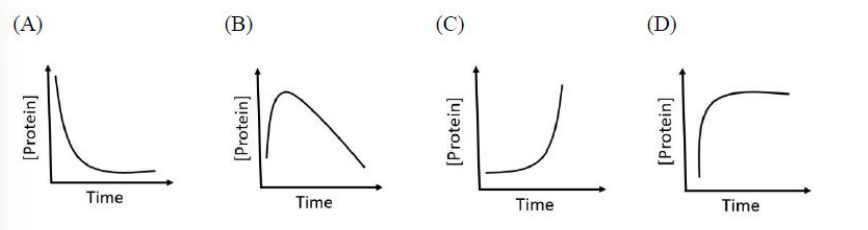
\includegraphics[width=0.8\textwidth]{figures/26.png}
\end{center}

\vspace{0.5cm}

\questionb{The distribution of marks scored by a large class in an exam can be represented as a normal distribution with mean $\mu$ and standard deviation $\sigma$. In a follow-up exam in the same class, everyone scored 5 marks more than their respective score in the earlier exam. For this follow-up exam, the distribution of marks can be represented as a normal distribution with mean $\mu_2$ and standard deviation $\sigma_2$. Which one of the following is correct?}{27}
\begin{enumerate}
    \item[(A)] $\mu = \mu_2; \sigma > \sigma_2$
    \item[(B)] $\mu < \mu_2; \sigma > \sigma_2$  
    \item[(C)] $\mu > \mu_2; \sigma < \sigma_2$
    \item[(D)] $\mu < \mu_2; \sigma = \sigma_2$
\end{enumerate}

\vspace{0.5cm}

\questionb{The angle (in degrees) between the vectors $\vec{x} = \hat{i} - \hat{j} + 2\hat{k}$ and $\vec{y} = 2\hat{i} - \hat{j} - 1.5\hat{k}$ is \_\_\_\_\_.}{28}

\vspace{0.5cm}

\questionb{Match the proteins in Group I with cellular processes in Group II}{29}

\begin{tabularx}{\linewidth}{|l|X|}
\hline
\textbf{Group I} & \textbf{Group II} \\
\hline
P. p53 & 1. DNA packaging \\
Q. Lysozyme & 2. Apoptosis \\
R. Tubulins & 3. Hydrolysis of polysaccharides \\
S. Histones & 4. Chromosome segregation \\
\hline
\end{tabularx}

\begin{enumerate}
    \item[(A)] P-4, Q-2, R-3, S-1
    \item[(B)] P-2, Q-3, R-1, S-4  
    \item[(C)] P-4, Q-3, R-1, S-2
    \item[(D)] P-2, Q-3, R-4, S-1
\end{enumerate}

\vspace{0.5cm}

\questionb{The circular dichroism spectra of three proteins P, Q, and R are given below:

\begin{center}
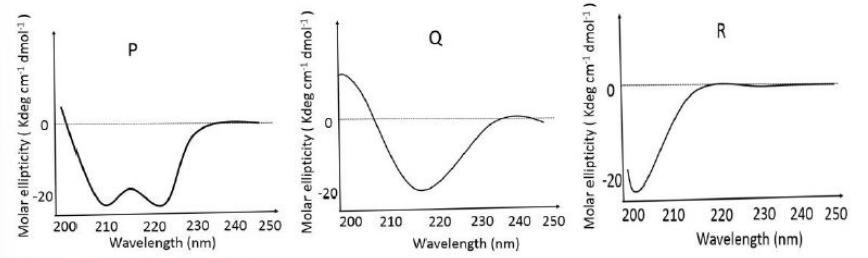
\includegraphics[width=0.8\textwidth]{figures/30.png}
\end{center}

Choose the correct combination.}{30}
\begin{enumerate}
    \item[(A)] P: $\alpha$-helix, Q: $\beta$-sheet, and R: Random coil
    \item[(B)] P: $\beta$-sheet, Q: $\alpha$-helix, and R: Random coil  
    \item[(C)] P: $\alpha$-helix, Q: Random coil, and R: $\beta$-sheet
    \item[(D)] P: Random coil, Q: $\alpha$-helix, and R: $\beta$-sheet
\end{enumerate}

\vspace{0.5cm}

\questionb{Match the organisms in Column I with the characteristics in Column II}{31}

\begin{tabularx}{\linewidth}{|l|X|}
\hline
\textbf{Column I} & \textbf{Column II} \\
\hline
P. Methanococcus & 1. Halophilic \\
Q. Dunaliella & 2. Acidophile \\
R. Sulfolobus & 3. Mesophile \\
S. Escherichia & 4. Barophile \\
\hline
\end{tabularx}

\begin{enumerate}
    \item[(A)] P-4, Q-3, R-2, S-1
    \item[(B)] P-3, Q-2, R-4, S-1  
    \item[(C)] P-2, Q-1, R-4, S-3
    \item[(D)] P-4, Q-1, R-2, S-3
\end{enumerate}

\vspace{0.5cm}

\questionb{Which one of the following amino acids has three ionizable groups?}{32}
\begin{enumerate}
    \item[(A)] Glycine
    \item[(B)] Leucine  
    \item[(C)] Valine
    \item[(D)] Lysine
\end{enumerate}

\vspace{0.5cm}

\questionb{Consider an infinite number of cylinders. The first cylinder has a radius of 1 meter and height of 1 meter. The second one has a radius of 0.5 meter and height of 0.5 meter. Every subsequent cylinder has half the radius and half the height of the preceding cylinder. The sum of the volumes (in cubic meters) of these infinite number of cylinders is \_\_\_\_\_.}{33}

\vspace{0.5cm}

\questionb{The concentration (in micromolar) of NADH in a solution with $A_{340} = 0.50$ is \_\_\_\_\_.}{34}

\vspace{0.5cm}

\questionb{The specific activity of an enzyme in a crude extract of \textit{E. coli} is 9.5 units/mg of protein. The specific activity increased to 68 units/mg of protein upon ion-exchange chromatography. The fold purification is \_\_\_\_\_.}{35}

\vspace{0.5cm}

\questionb{Which one of the following organisms is responsible for crown gall disease in plants?}{36}
\begin{enumerate}
    \item[(A)] \textit{Xanthomonas campestris}
    \item[(B)] \textit{Rhizobium eili}  
    \item[(C)] \textit{Agrobacterium tumefaciens}
    \item[(D)] \textit{Erwinia stewartii}
\end{enumerate}

\vspace{0.5cm}

\questionb{The value of $c$ for which the following system of linear equations has an infinite number of solutions is \_\_\_\_\_.}{37}

\[
\begin{bmatrix}
1 & 2 \\
1 & 2 
\end{bmatrix}
\begin{bmatrix}
x \\
y 
\end{bmatrix}
= 
\begin{bmatrix}
c \\
4 
\end{bmatrix}
\]

\vspace{0.5cm}

\questionb{Match the plant hormones in Column I with functions in Column II}{38}

\begin{tabularx}{\linewidth}{|l|X|}
\hline
\textbf{Column I} & \textbf{Column II} \\
\hline
P. Gibberellic acid & 1. Seed and bud dormancy \\
Q. Zeatin & 2. Fruit ripening \\
R. Ethylene & 3. Delaying leaf senescence \\
S. Abscisic acid & 4. Regulation of plant height \\
\hline
\end{tabularx}

\begin{enumerate}
    \item[(A)] P-4, Q-3, R-2, S-1
    \item[(B)] P-4, Q-2, R-3, S-1  
    \item[(C)] P-3, Q-1, R-2, S-4
    \item[(D)] P-2, Q-1, R-4, S-3
\end{enumerate}

\vspace{0.5cm}

\questionb{For an \textit{E. coli} culture in the exponential phase of growth, optical density (OD) at 540 nm is 0.3 at 2 hours and 0.6 at 4 hours. Assuming that the measured OD is linearly proportional to the number of \textit{E. coli} cells, the growth rate (per hour) for this culture is \_\_\_\_\_.}{39}

\vspace{0.5cm}

\questionb{An immunocompetent person becomes infected with a pathogenic strain of bacteria. Which one of the following graphs correctly depicts bacterial load in this person over time?}{40}

\begin{center}
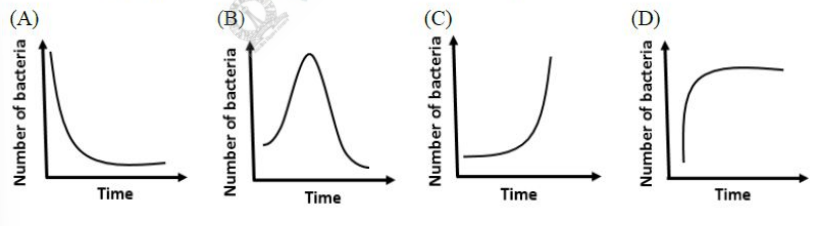
\includegraphics[width=0.8\textwidth]{figures/40.png}
\end{center}

\vspace{0.5cm}

\questionb{The genome is diploid at the end of which phases of a human mitotic cell cycle?}{41}
\begin{enumerate}
    \item[(A)] G2 \& S
    \item[(B)] G1 \& M  
    \item[(C)] M \& S
    \item[(D)] G1 \& G2
\end{enumerate}

\vspace{0.5cm}

\questionb{A recombinant protein is to be expressed under the control of the \textit{lac} promoter and operator in a strain of \textit{E. coli} having the genotype \textit{lacI$^+$ crp$^+$}. Even in the absence of inducer IPTG, low levels of expression of the recombinant protein are seen (leaky expression). Which one of the following should be done to minimize such leaky expression?}{42}
\begin{enumerate}
    \item[(A)] Addition of lactose to the medium
    \item[(B)] Removal of all glucose from the medium  
    \item[(C)] Addition of excess glucose to the medium
    \item[(D)] Addition of \textit{allo}-lactose to the medium
\end{enumerate}

\vspace{0.5cm}

\questionb{Shown below is a plasmid vector (P) and an insert (Q). The insert was cloned into the \textit{BamH1} site of the vector. The recombinant plasmid was isolated and digested with \textit{BamH1} or \textit{Xho1}. The results from the digestion experiments are shown in (R).

\begin{center}
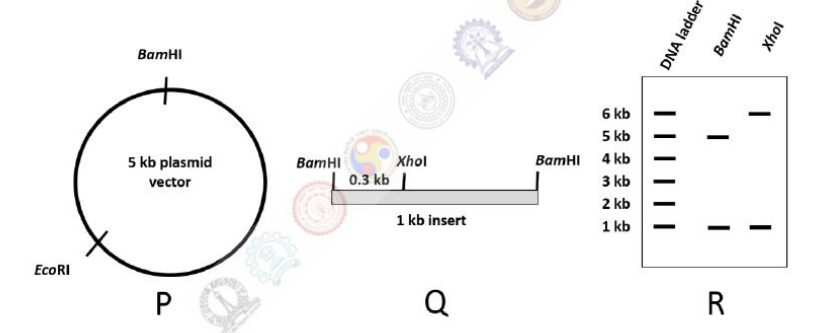
\includegraphics[width=0.8\textwidth]{figures/43.png}
\end{center}

Which one of the following explains the digestion results shown in (R)?}{43}
\begin{enumerate}
    \item[(A)] The insert did not ligate to the vector.
    \item[(B)] One copy of the insert ligated to the vector.  
    \item[(C)] The insert ligated to the vector as two tandem copies.
    \item[(D)] The insert ligated to the vector as two copies but not in tandem.
\end{enumerate}

\vspace{0.5cm}

\questionb{Which one of the following CANNOT be a recognition sequence for a Type II restriction enzyme?}{44}
\begin{enumerate}
    \item[(A)] GAATTC
    \item[(B)] AGCT  
    \item[(C)] GCGGCCGC
    \item[(D)] ATGCCT
\end{enumerate}

\vspace{0.5cm}

\questionb{A pedigree of an inheritable disease is shown below.

\begin{center}
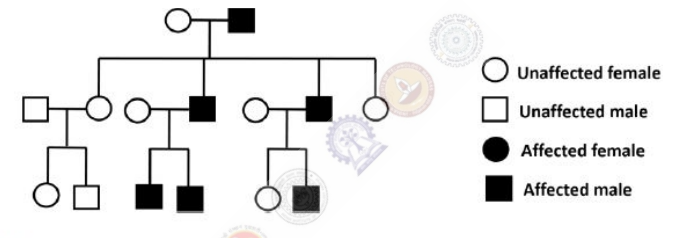
\includegraphics[width=0.7\textwidth]{figures/45.png}
\end{center}

This inheritable disease is}{45}
\begin{enumerate}
    \item[(A)] X-linked dominant
    \item[(B)] X-linked recessive or Y-linked  
    \item[(C)] only Y-linked
    \item[(D)] only X-linked recessive
\end{enumerate}

\vspace{0.5cm}

\questionb{If the chemical composition of proteins in an organism is CH\textsubscript{1}SO\textsubscript{3}N\textsubscript{0.3}S\textsubscript{0.004}, the mass percentage of carbon in the proteins is \_\_\_\_\_.}{46}

\vspace{0.5cm}

\questionb{For the probability density P(x) = 0.5e\textsuperscript{-0.5x}, the integral $\int_{0}^{\infty} P(x)dx$ = \_\_\_\_\_.}{47}

\vspace{0.5cm}

\questionb{Growth of a microbe in a test tube is modeled as $\frac{dx}{dt} = rX \left(1 - \frac{x}{K}\right)$, where, X is the biomass, r is the growth rate, and K is the carrying capacity of the environment ($r \neq 0$; $K \neq 0$). If the value of starting biomass is $\frac{K}{100}$, which one of the following graphs qualitatively represents the growth dynamics?}{48}
\begin{center}
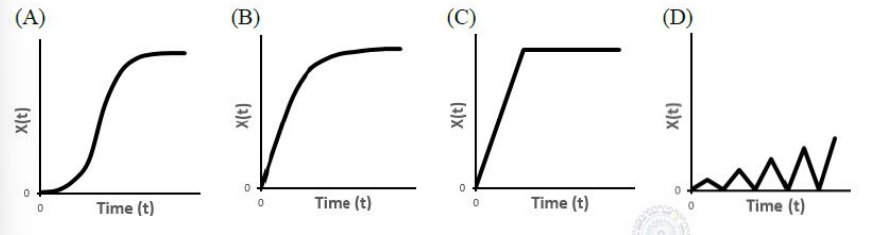
\includegraphics[width=0.8\textwidth]{figures/48.png}
\end{center}

\vspace{0.5cm}

\questionb{A zero-order liquid phase reaction A$\rightarrow$B is being carried out in a batch reactor with $k = 10^{-3}$ mol/min. If the starting concentration of A is 0.1 moles/liter, the time (in minutes) taken by the system before A is exhausted in a 100 liter reactor is \_\_\_\_\_.}{49}

\vspace{0.5cm}

\questionb{The interaction energy E between two spherical particles is plotted as a function of the distance (r) between them. When r$<$a, where a is a constant, the net force between the spherical particles is repulsive. When r$>$a, they attract via van der Waals attraction. Which one of the following plots correctly represents the interaction energy between the above two particles?}{50}

\begin{center}
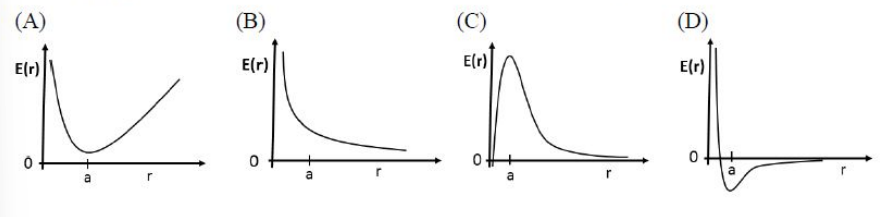
\includegraphics[width=0.8\textwidth]{figures/50.png}
\end{center}

\vspace{0.5cm}

\questionb{EcoRI restriction sites on a 10kb DNA fragment are shown below:

\begin{center}
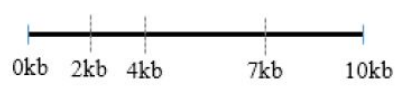
\includegraphics[width=0.7\textwidth]{figures/51.png}
\end{center}

Upon partial digestion, what are the lengths (in kb) of all the possible DNA fragments obtained?}{51}
\begin{enumerate}
    \item[(A)] 2, 3, 4, 5, 6, 7, 8, and 10
    \item[(B)] 2, 3, 4, 5, 6, and 7  
    \item[(C)] 2, 3, 4, and 7
    \item[(D)] 2 and 3
\end{enumerate}

\vspace{0.5cm}

\questionb{A DNA strand of length 25 nm wraps diametrically around the circumference of a spherical histone-octamer once. The radius (nm) of the histone-octamer is \_\_\_\_\_.}{52}

\vspace{0.5cm}

\questionb{One hundred E. coli cells are each infected by a single $\lambda$ phage particle. The ratio of the number of phage particles committing to lysogeny to those committing to lysis is 4:1. Assuming that the average burst size is 80, the number of free phage particles released after one round of infection is \_\_\_\_\_.}{53}

\vspace{0.5cm}

\questionb{During anaerobic growth, an organism converts glucose (P) into biomass (Q), ethanol (R), acetaldehyde (S), and glycerol (T). Every mole of carbon present in glucose gets distributed among the products as follows:

\[1 \, (\text{C-mole P}) \rightarrow 0.14 \, (\text{C-mole Q}) + 0.25 \, (\text{C-mole R}) + 0.3 \, (\text{C-mole S}) + 0.31 \, (\text{C-mole T})\]

From 1800 grams of glucose fed to the organism, the ethanol produced (in grams) is \_\_\_\_\_.}{54}

\vspace{0.5cm}

\questionb{Which of the following conditions promote the development of human autoimmune disorders?}{55}
\begin{enumerate}
\item[P.] Inability to eliminate self-reactive lymphocytes  
\item [Q.] Generation of auto-antibodies  
\item [R.] Ability to eliminate self-reactive T-cells  
\item [S.] Induction of regulatory T-cells in the thymus 
\end{enumerate}

\begin{enumerate}
    \item[(A)] P, R
    \item[(B)] Q, S  
    \item[(C)] P, Q
    \item[(D)] R, S
\end{enumerate}

\vspace{0.5cm}

\vspace{5cm}
\begin{center}
\textbf{END OF THE QUESTION PAPER}
\rule{\textwidth}{0.5pt} 
\end{center}

\end{document}